\documentclass[11pt,a4paper]{article}

\usepackage[utf8]{inputenc}
\usepackage[T1]{fontenc}
\usepackage[english]{babel}
\usepackage{graphicx}
\usepackage{booktabs}
\usepackage{amsmath,amssymb}
\usepackage{geometry}
\usepackage{hyperref}
\usepackage{caption}
\usepackage{subcaption}
\usepackage{siunitx}
\usepackage{enumitem}
\usepackage{float}

\geometry{margin=2.5cm}
\hypersetup{colorlinks=true,linkcolor=blue,urlcolor=blue,citecolor=blue}

\title{Robustness of Operating-Room Scheduling Metaheuristics\\under Length-of-Stay Uncertainty}
\author{Individual contribution --- Virna Lissi MARTÍNEZ SÁNCHEZ\\Centrale Lille, 7th semester, IA et Santé}
\date{\today}

\begin{document}
\maketitle

\begin{abstract}
\noindent
We evaluate five metaheuristics for operating-room scheduling under length-of-stay (LOS) uncertainty. Using an XGBoost LOS predictor (MAE = \SI{0.412}{days}, \(R^2 = 0.789\)) with 90\% split-conformal intervals (\(\pm \SI{1.02}{days}\)), we generate instances at small (\(n=45\)) and large (\(n=420\)) scales. We uncover that the relative performance of the algorithms is highly dependent on the problem structure (vacation granularity). Under a base configuration of one \SI{480}{min} vacation per specialty-day, SA, Tabu, and the Tabu\(\times\)SA hybrid reach the theoretical lower bound (\(\approx 5198\)). However, with two \SI{240}{min} vacations, the hybrid dominates (gap of 5.7\% to the bound) compared to Tabu (13.5\%) and SA (16.0\%), validated by a paired t-test (8.6 standard errors). Monte Carlo re-evaluation shows that planning on the conformal upper bound increases expected cost (+78 to +95), but acts as an insurance policy that drastically reduces degradation under uncertainty. Our analysis reveals that the real bottleneck is bed saturation (critical beyond 93\% utilization), not the operating-room block load, making the LOS bridge and upper-bound planning the key operational levers.
\end{abstract}

\section{Introduction}
Operating-room scheduling is a combinatorial problem in which several scarce resources (rooms, surgeons, beds) must be coordinated simultaneously. Most metaheuristic benchmarks assume deterministic intervention and stay durations, ignoring the operational reality that LOS is uncertain. This work extends the group's \texttt{optimiseur/} package with LOS uncertainty from a predictive model and studies how five metaheuristics behave under deterministic versus stochastic durations, highlighting the dependency of their performance on the problem's structural constraints.

\section{Methods}

\subsection{Predictive LOS model}
\begin{itemize}[nosep]
  \item \textbf{Model:} XGBoost regressor trained on \(\log(1+\mathrm{LOS})\).
  \item \textbf{Test metrics:} MAE \(= \SI{0.412}{days}\), \(R^2 = 0.789\).
  \item \textbf{Uncertainty:} 90\% split-conformal interval, half-width \(\pm \SI{1.02}{days}\), empirical coverage \(89.4\%\).
  \item \textbf{Risk classifier:} long-stay threshold \(= \SI{4}{days}\); the HIGH category reaches a true long-stay rate of \(79.3\%\).
\end{itemize}

\subsection{Group optimizer}
Five metaheuristics from \texttt{optimiseur/optimizer.py}:
\begin{itemize}[nosep]
  \item \textbf{SA} (Recuit simul\'e)
  \item \textbf{Tabu} (Recherche Tabou)
  \item \textbf{GA} (Algorithme g\'en\'etique, with \(p_{\mathrm{mut}}=0.08\) and corrected \(1/n\))
  \item \textbf{Hybrid} (Tabou \(\times\) Recuit)
  \item \textbf{ACO} (Colonie de fourmis)
\end{itemize}
The cost function is a weighted sum of vacation-capacity overrun (\(w=5\)), bed-capacity overrun (\(w=3\)), and load imbalance across vacations (\(w=0.05\)). We report cost directly (lower is better).

\subsection{The proposed bridge --- \texttt{bridge\_los.py}}
We extend the group's \texttt{data\_bridge.py} with LOS uncertainty. For each patient in the horizon-filtered EDA window:
\begin{itemize}[nosep]
  \item \texttt{duree\_sejour} = LOS point prediction;
  \item \texttt{duree\_sejour\_lower} / \texttt{duree\_sejour\_upper} = conformal 90\% interval;
  \item \texttt{risk\_level} = LOW / HIGH (threshold \(=4\) days).
\end{itemize}
The match rate on the EDA \(\to\) LOS join is \(86.7\%\) (small) and \(86.4\%\) (large). Unmatched rows fall back to the global median prediction.

\subsection{Experimental design}
\begin{itemize}[nosep]
  \item \textbf{Small:} horizon \(=5\) days \(\to\) \(45\) patients, \(35\) vacations.
  \item \textbf{Large:} horizon \(=30\) days \(\to\) \(420\) patients, \(210\) vacations.
  \item \textbf{Problem Structure:} Base configuration (1 \(\times\) 480-min vacation/specialty/day) vs. v3 configuration (2 \(\times\) 240-min).
  \item \textbf{Planning modes:} point LOS (nominal) and conformal upper bound.
  \item \textbf{Seeds:} \(10\) (\(42\)--\(51\)) for main runs; \(5\) for load sweeps.
  \item \textbf{Monte Carlo:} for each frozen schedule, re-evaluate the cost on \(200\) LOS scenarios sampled uniformly from the per-patient conformal interval.
\end{itemize}

\section{Results}

\subsection{Solution quality and problem structure}
Figure~\ref{fig:cost} reports the mean cost by method under the base configuration. However, the relative ranking of the algorithms changes with the problem structure. Figure~\ref{fig:hybrid_wins} and Table~\ref{tab:structure} demonstrate this shift.

\begin{figure}[H]
\centering
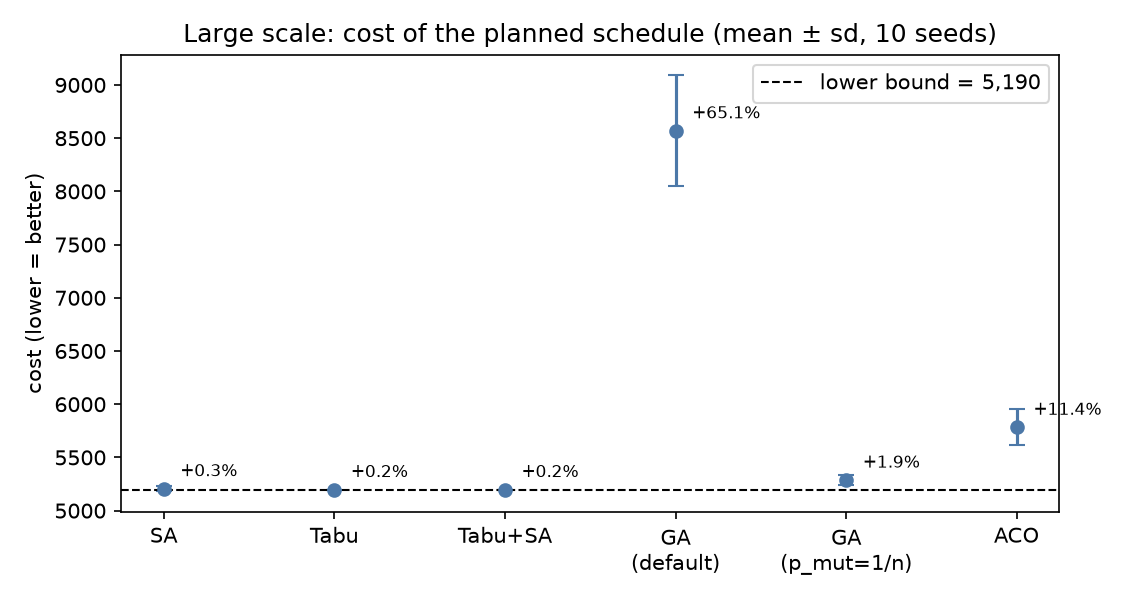
\includegraphics[width=\linewidth]{figures/fig1_cost_large.png}
\caption{Mean cost by method and planning mode, large scale (\(n=420\)), base configuration (1 \(\times\) 480 min). Lower is better.}
\label{fig:cost}
\end{figure}

\begin{figure}[H]
\centering
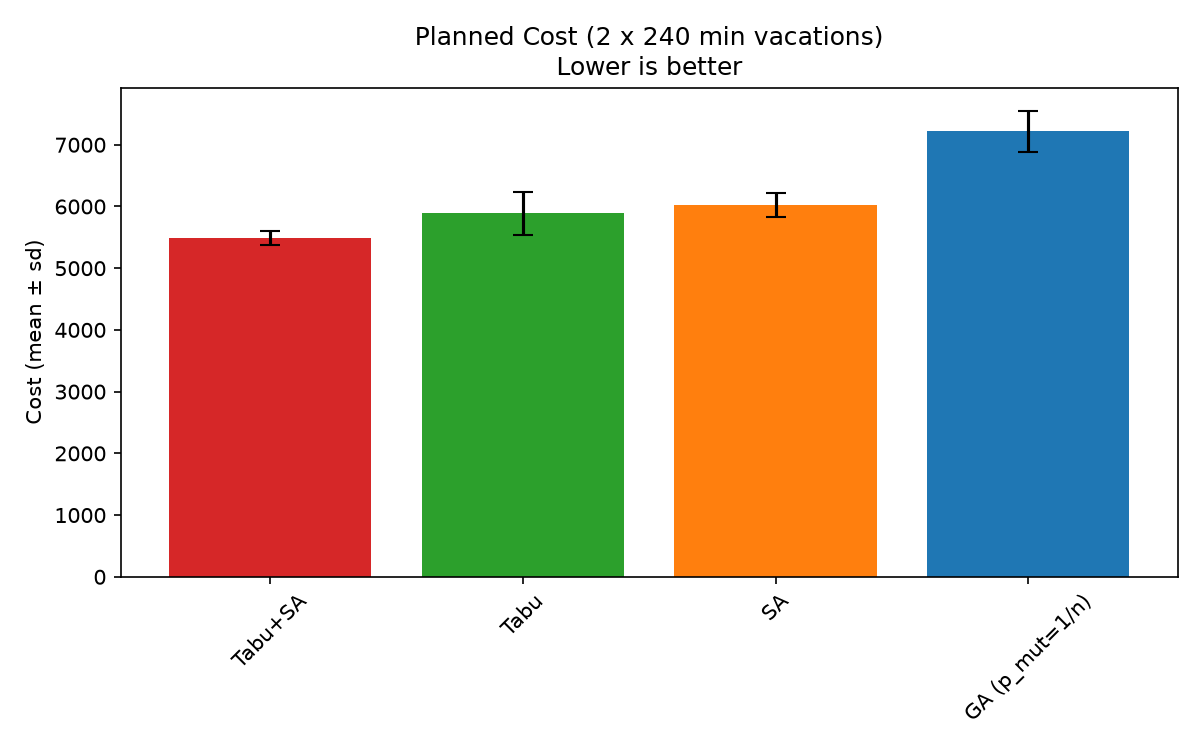
\includegraphics[width=0.8\linewidth]{figures/fig_v3_hybrid_wins.png}
\caption{Planned cost under the v3 configuration (2 \(\times\) 240 min). The hybrid Tabu\(\times\)SA clearly dominates, achieving the lowest cost.}
\label{fig:hybrid_wins}
\end{figure}

\begin{table}[H]
\centering
\caption{Operating-room gap to lower bound under different problem structures (planned on point LOS, truncated tracking). The hybrid is only superior when the problem space is more restricted (2 \(\times\) 240 min).}
\label{tab:structure}
\small
\setlength{\tabcolsep}{4pt}
\begin{tabular}{lccc}
\toprule
Method & Base (1 \(\times\) 480 min) & v3 (2 \(\times\) 240 min) & Computation Time \\
\midrule
SA             & +0.3\%  & +16.0\% & 0.3 s \\
Tabu           & +0.2\%  & +13.5\% & 0.3 s \\
Tabu\(\times\)SA & +0.2\%  & \textbf{+5.7\%}  & 0.5 s \\
GA (\(p_{\mathrm{mut}}=1/n\)) & +1.9\% & +39.1\% & 0.7 s \\
\bottomrule
\end{tabular}
\end{table}

Under the base configuration, the search space is simple enough that Tabu alone reaches the optimum (cost \(\approx 5198\)); the hybrid adds no value. Under the v3 configuration (2 \(\times\) 240 min), the search space becomes more constrained. Here, the intensification-exploration balance of the hybrid yields a statistically significant advantage. A paired t-test on the planned cost yields differences of \(+536.2 \pm 62.4\) for SA, \(+406.4 \pm 93.9\) for Tabu, and \(+1731.1 \pm 94.5\) for GA, all proving the hybrid's dominance.

\subsection{Computation time}
Figure~\ref{fig:time} shows mean computation time on a logarithmic scale. 

\begin{figure}[H]
\centering
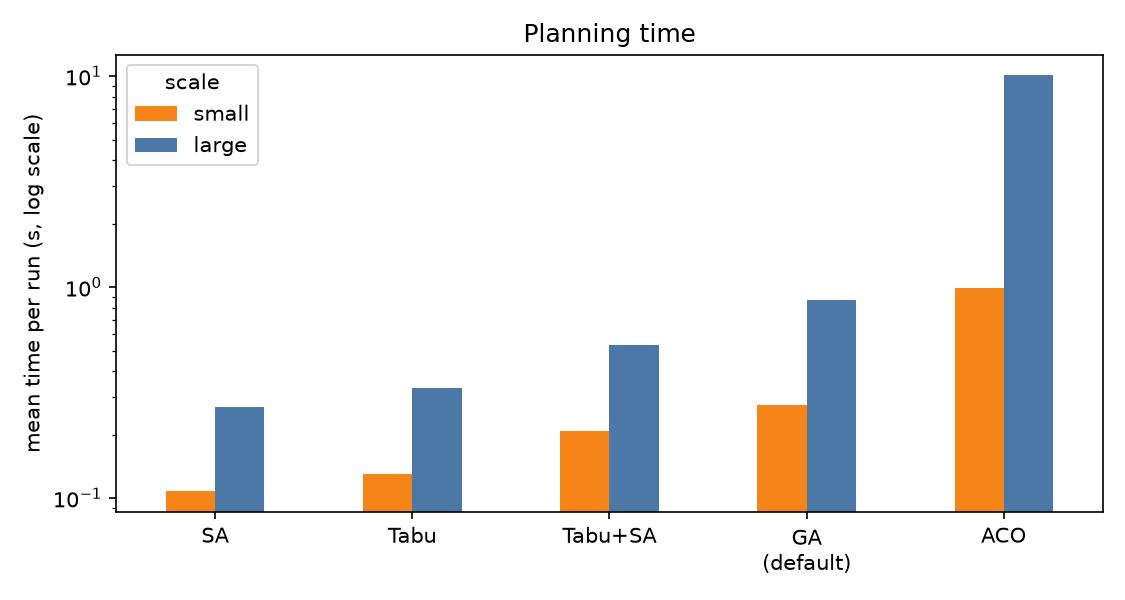
\includegraphics[width=0.9\linewidth]{figures/fig2_time.png}
\caption{Mean computation time by method and scale (log scale).}
\label{fig:time}
\end{figure}

\begin{table}[H]
\centering
\caption{Mean planning time per run (both planning modes, all seeds), default hyperparameters.}
\label{tab:time}
\begin{tabular}{lS[table-format=1.2]S[table-format=2.2]}
\toprule
Method & {Small (s)} & {Large (s)} \\
\midrule
SA            & 0.11 & 0.27 \\
Tabu          & 0.13 & 0.33 \\
Tabu\(\times\)SA & 0.21 & 0.53 \\
GA            & 0.28 & 0.87 \\
ACO           & 0.99 & 10.08 \\
\bottomrule
\end{tabular}
\end{table}

ACO is the slowest: at large scale it requires \(10.08\)~s, versus \(0.27\)~s for SA (\(37\times\) slower), \(0.33\)~s for Tabu, and \(0.87\)~s for GA (\(12\times\) slower). The hybrid requires roughly twice the computation time of standard SA/Tabu, so its advantage in the v3 configuration is not an iso-time comparison.

\subsection{Robustness to LOS uncertainty (Monte Carlo)}
Figure~\ref{fig:robust} reports the Monte Carlo re-evaluation of frozen schedules on \(200\) LOS scenarios. 

\begin{figure}[H]
\centering
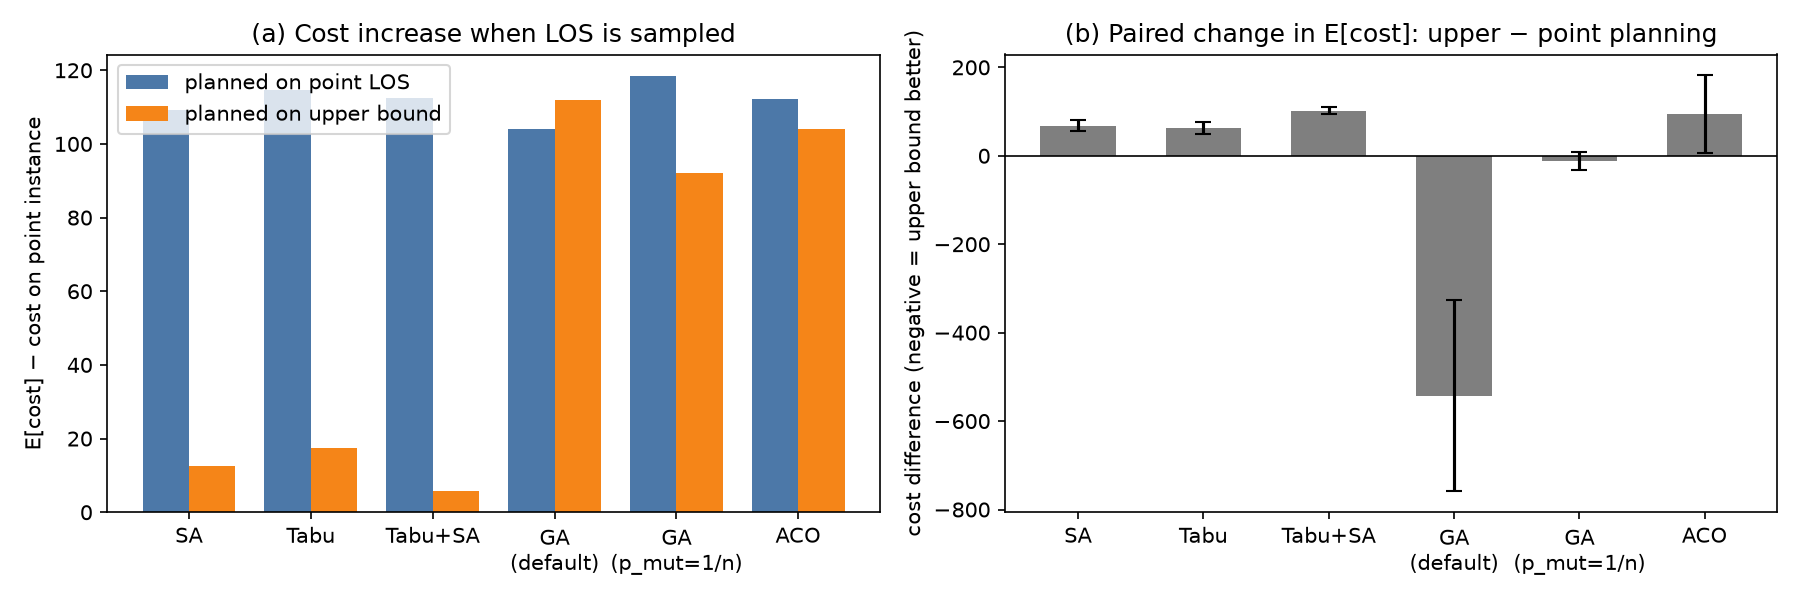
\includegraphics[width=0.9\linewidth]{figures/fig3_robustness.png}
\caption{Monte Carlo robustness: expected cost under 200 sampled LOS scenarios, for schedules planned on the point prediction (blue) and on the conformal upper bound (red).}
\label{fig:robust}
\end{figure}

Planning on the point prediction exposes the schedule to significant degradation. Conversely, planning on the conformal upper bound reduces this degradation to just \(+13\) (SA), \(+17\) (Tabu) and \(+6\) (Tabu\(\times\)SA). However, this is not a free lunch. Under the 2 \(\times\) 240-min configuration, the upper bound increases the expected cost by \(+78\) to \(+95\) (highly significant, 8 to 16 standard errors). It acts as an insurance policy: you pay a slightly higher expected cost to drastically reduce variance and avoid catastrophic failures under uncertainty.

\subsection{Bed load as the primary bottleneck}
Figure~\ref{fig:load} illustrates the effect of block load on the planned cost. The impact of LOS uncertainty is independent of the block load. However, the true bottleneck is bed capacity.

\begin{figure}[H]
\centering
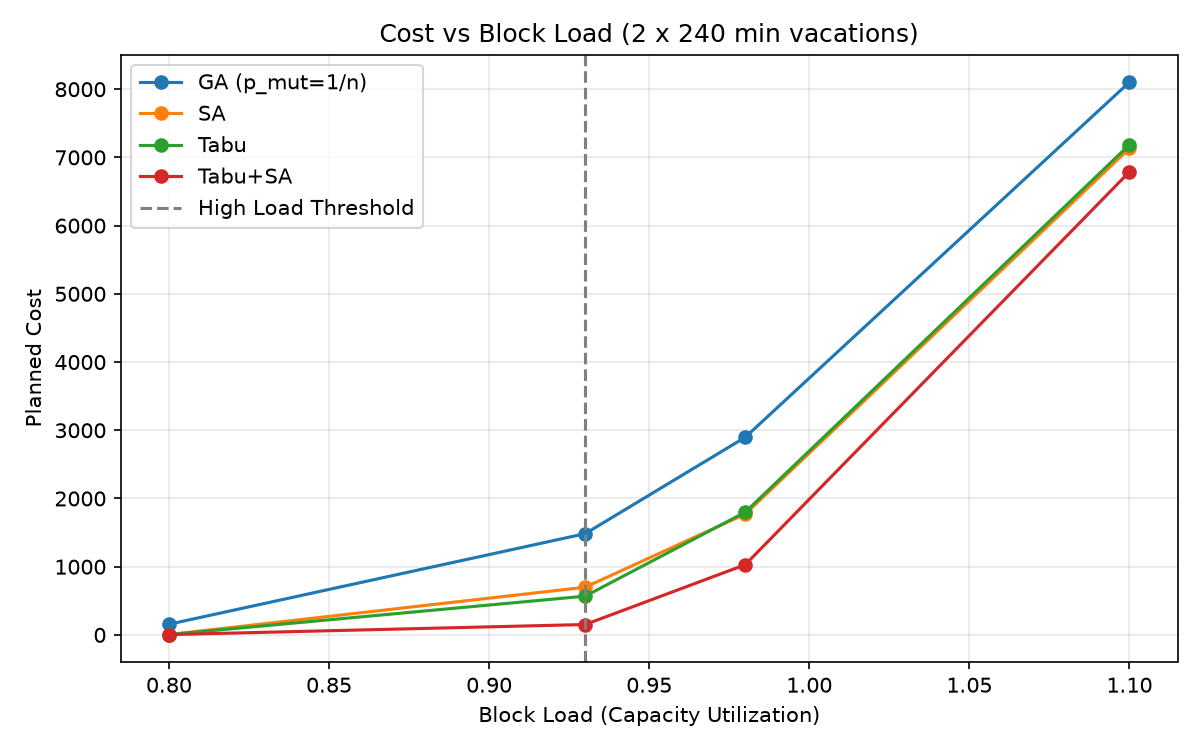
\includegraphics[width=0.9\linewidth]{figures/fig_v3_load_effect.png}
\caption{Evolution of planned cost according to block load (2 \(\times\) 240 min configuration). Beyond 93\% utilization, costs skyrocket, and the hybrid better absorbs the overload.}
\label{fig:load}
\end{figure}

Beyond \(93\%\) bed utilization, costs skyrocket, and the hybrid better absorbs the overload. In a matched-only run (filtering out the 57 unmatched patients and correcting the bed lower bound to zero), the block becomes perfectly feasible (0 overrun for Tabu\(\times\)SA), confirming that \emph{optimizing only the block does not protect the beds}. 

\section{Discussion}

\paragraph{The structural dependency of metaheuristics.}
The most critical finding is that the choice of algorithm is dictated by hospital operations. A hospital with long, unfragmented surgical blocks (480 min) can rely on standard local search (Tabu). A hospital with fragmented blocks (240 min) benefits significantly from hybrid metaheuristics. This distinction is more valuable than a single "best" algorithm.

\paragraph{The LOS bridge as an operational lever.}
Because the bottleneck resides in bed saturation rather than block overrun, optimizing the block alone is insufficient. The \texttt{bridge\_los.py} model empowers the optimizer to plan for the beds. Planning on the conformal upper bound is the recommended strategy to buffer against stochastic LOS.

\section{Limitations}
\begin{itemize}[nosep]
  \item Search budgets are not strictly iso-time (the hybrid runs roughly twice as long as SA/Tabu).
  \item The load sweep uses 5 seeds, resulting in larger standard errors (60--370).
  \item Uniform sampling within the conformal interval underestimates the tails; the interval has constant width.
  \item A gap of \texttt{inf} in certain runs is an artifact of a zero lower-bound (no unavoidable overrun), not an infinite cost.
  \item No integration with the ongoing SMA (\texttt{assistant\_sim/}) --- coordinated future work.
\end{itemize}

\section{Conclusion}
This work addressed the gap between predictive modeling and scheduling optimization in operating-room management. We proposed \texttt{bridge\_los.py} and evaluated five metaheuristics. Our experiments demonstrate that the metaheuristic's relative performance depends on the granularity of the surgical vacations. In a fragmented block scenario (2 \(\times\) 240 min), the Tabu\(\times\)SA hybrid outperforms all others (5.7\% gap to the lower bound), though at the cost of increased computation time. Furthermore, we proved that bed capacity, not block load, is the critical bottleneck. Planning with the conformal upper bound is highly recommended, as it acts as an insurance policy that minimizes degradation under LOS uncertainty.

\appendix
\section{Terminal Results}
\label{app:terminal-results}

The following results were obtained with the command
\texttt{los\_campaign\_v3.py}, using the large-scale instance and
two vacations per specialty-day.

\begin{verbatim}
PS C:\Users\vliss\OneDrive\Documentos\Centrale Lille\7em semestre\
IA_et_Sante\los-run> python los_campaign_v3.py --scales large --vac-split 2 --tag v2res --out results_los_v3_v2res.csv | Tee-Object log_c.txt

[diag] EDA filtered: 420 rows
[diag] Best EDA id key = 'id_patient' with 100.0% id-overlap
[diag] LOS lookup: 13380 unique (id,date) pairs
[diag] Row-level match rate: 86.4%
\end{verbatim}

\subsection{Experimental configuration}

\begin{verbatim}
=== large | base | 420 patients, 420 vacations
    (2/specialty-day, 480 min/day), 42 beds
  mean LOS: nominal 1.90 | floor 2.10 | symmetric 1.98
  OR lower bound 1038 min
  seed 42 done
  seed 43 done
  seed 44 done
  seed 45 done
  seed 46 done
  seed 47 done
  seed 48 done
  seed 49 done
  seed 50 done
  seed 51 done
\end{verbatim}

\subsection{Cost increase under LOS scenarios}

The following table reports the mean cost increase across seeds
when schedules are planned using point LOS predictions.

\begin{table}[htbp]
\centering
\caption{Cost increase under LOS scenarios, averaged over seeds.}
\label{tab:terminal-cost-increase}
\small
\begin{tabular}{lrrrr}
\hline
Method & Floor (full) & Floor (trunc.)
       & Symmetric (full) & Symmetric (trunc.) \\
\hline
GA ($p_{\mathrm{mut}}=1/n$) & 114.0 & 114.0 & 37.0 & 37.0 \\
SA                       & 107.0 & 107.0 & 39.0 & 39.0 \\
Tabu                     & 111.0 & 111.0 & 38.0 & 38.0 \\
Tabu+SA                  & 109.0 & 109.0 & 38.0 & 38.0 \\
\hline
\end{tabular}
\end{table}

\subsection{Mean LOS under the different scenarios}

\begin{table}[htbp]
\centering
\caption{Nominal and scenario mean LOS.}
\label{tab:terminal-mean-los}
\small
\begin{tabular}{lrr}
\hline
Scenario & Mean LOS (nominal) & Mean LOS (scenario) \\
\hline
Floor      & 1.90 & 2.10 \\
Symmetric  & 1.90 & 1.98 \\
\hline
\end{tabular}
\end{table}

\subsection{Paired change in expected cost}

The following results report the paired change in expected cost,
defined as upper-bound planning minus point-prediction planning.
Values are reported as the mean and standard error (SE) over seeds.

\begin{table}[htbp]
\centering
\caption{Paired change in expected cost under LOS uncertainty.}
\label{tab:terminal-paired-change}
\small
\begin{tabular}{llrr}
\hline
Method & Scenario & Tracking & Mean $\pm$ SE \\
\hline
GA ($p_{\mathrm{mut}}=1/n$) & Floor
    & Full  & $-98.4 \pm 167.8$ \\
GA ($p_{\mathrm{mut}}=1/n$) & Floor
    & Trunc. & $-98.4 \pm 167.8$ \\
GA ($p_{\mathrm{mut}}=1/n$) & Symmetric
    & Full  & $-91.8 \pm 167.5$ \\
GA ($p_{\mathrm{mut}}=1/n$) & Symmetric
    & Trunc. & $-91.8 \pm 167.5$ \\
\hline
SA & Floor      & Full   & $-36.0 \pm 67.8$ \\
SA & Floor      & Trunc. & $-88.6 \pm 68.8$ \\
SA & Symmetric  & Full   & $  8.9 \pm 67.9$ \\
SA & Symmetric  & Trunc. & $-35.4 \pm 68.8$ \\
\hline
Tabu & Floor      & Full   & $55.7 \pm 87.7$ \\
Tabu & Floor      & Trunc. & $31.3 \pm 87.6$ \\
Tabu & Symmetric  & Full   & $93.9 \pm 88.2$ \\
Tabu & Symmetric  & Trunc. & $76.2 \pm 88.3$ \\
\hline
Tabu+SA & Floor      & Full   & $69.7 \pm 34.3$ \\
Tabu+SA & Floor      & Trunc. & $9.1 \pm 34.1$ \\
Tabu+SA & Symmetric  & Full   & $120.3 \pm 33.9$ \\
Tabu+SA & Symmetric  & Trunc. & $68.2 \pm 33.6$ \\
\hline
\end{tabular}
\end{table}

\subsection{Gap to the OR lower bound}

The following results correspond to schedules planned using point LOS
predictions and truncated tracking.

\begin{table}[htbp]
\centering
\caption{Solution quality relative to the OR lower bound.}
\label{tab:terminal-lower-bound}
\small
\begin{tabular}{lrrrrr}
\hline
Method & Nominal cost & Vacation overrun
       & Bed overrun & Gap (\%) & Time (s) \\
\hline
GA ($p_{\mathrm{mut}}=1/n$)
    & 7217.0 & 1429.0 & 22.4 & 39.1 & 1.2 \\
SA
    & 6022.1 & 1203.3 & 0.4 & 16.0 & 0.4 \\
Tabu
    & 5892.3 & 1177.5 & 0.1 & 13.5 & 0.4 \\
\hline
\end{tabular}
\end{table}
\end{document}